\question Let $G = (V,E)$ be a graph. Recall that a function $c: V \to \{1,\ldots, k\}$ is a $k$-colouring if $c(u) \neq c(v)$ for every pair of adjacent vertices $u$ and $v$. For $1 \leq i \leq k$, the set $C_i = \{i \in V: c(u) = i\}$ is called a \emph{colour set} of $c$. For a pair $i,j$ with $1 \leq i < j \leq k$, let $G[i,j]$ denote the subgraph of $G$ induced by the set $C_i \cup C_j$. 

We say that a $k$-colouring $c$ of $G$ is \emph{safe} if for every pair $i,j$ with $i \neq j$, the subgraph $G[i,j]$ has maximum degree at most $3$. The \emph{safety number} of $G$ is the smallest number $k$ such that $G$ has a safe $k$-colouring.

Let \textsc{Safety Number} be the problem of deciding if a given graph $G$ has safety number at most $k$ for some given integer $k$. If $k$ is fixed (so if $k$ is not part of the input), then we denote the problem as \textsc{$k$-Safety Number}.

\begin{parts}
    \part[10] Basics

Among one million coins one erroneously shows ``heads'' on both sides; all other coins are fine. Suppose you pick one of those one million coins uniformly at random and toss it twenty times. Further suppose that it shows ``heads'' every single time. What is the probability that it's one of the good coins? Show your work and provide a numerical approximation.

\begin{solution}
    First, we introduce a needed result.
    \vspace{0.5em}
    \begin{theorem}[Bayes' theorem]
        Let $(\Omega, \Pr)$ be a finite discrete probability space and $A, B \subset \Omega$ events with $\Pr(B) > 0$. Then
        \[ \Pr[A \mid B] = \frac{\Pr[B \mid A] \cdot \Pr[A]}{\Pr[B]}. \]
    \end{theorem}
    \begin{proof}
        Consider the definition of conditional probability:
        \begin{equation} \label{eq:1}
            \Pr[A \mid B] = \frac{\Pr[A \cap B]}{\Pr[B]}.
        \end{equation}
        We similarly have
        \begin{equation} \label{eq:2}
            \Pr[B \mid A] = \frac{\Pr[A \cap B]}{\Pr[A]}.
        \end{equation}
        Rearranging (\ref{eq:2}) yields
        \[ \Pr[A \cap B] = \Pr[B \mid A] \Pr[A] \]
        and substituting this into (1) yields
        \[ \Pr[A \mid B] = \frac{\Pr[B \mid A] \cdot \Pr[A]}{\Pr[B]} \]
        as required.
    \end{proof}
    Let $A$ be the event that we pick a good coin, and $B$ be the event that our picked coin shows ``heads'' every time. Note $\overline A$ is the event we pick the erroneous coin. We are looking for $\Pr[A \mid B]$, which we can find using Bayes' theorem.
    We have
    \begin{align*}
        \Pr[A]        & = 1 - 10^{-6}, \\
        \Pr[B \mid A] & = 2^{-20}.
    \end{align*}
    We have left to find $\Pr[B]$, but we have
    \[ \Pr[B] = \Pr[B \mid A] \Pr[A] + \Pr[B \mid \overline A] \Pr[\overline A] \]
    by the law of total probabilities (as $\{A, \overline A\}$ form a partition of our sample set). We have
    \begin{align*}
        \Pr[\overline A]        & = 10^{-6}, \\
        \Pr[B \mid \overline A] & = 1.
    \end{align*}
    thus
    \[ \Pr[B] = 2^{-20}(1 - 10^{-6}) + 10^{-6}. \]
    We can now apply Bayes' theorem:
    \begin{align*}
        \Pr[A \mid B] & = \frac{\Pr[B \mid A] \cdot \Pr[A]}{\Pr[B]}                            \\
                      & = \frac{(2^{-20}) \cdot (1 - 10^{-6})}{2^{-20}(1 - 10^{-6}) + 10^{-6}} \\
                      & = 0.488
    \end{align*}
    correct to 3 significant figures.
\end{solution}

\part Tail bounds

Consider the digits in your CIS username as an integer number $C$, e.g., if your username were ``kqlz36'' then that would be $C = 36$. If you find $C < 10$ then instead let $C = 17$. Let $p = 1/C$. Consider the independent random variables $X_1, X_2, \ldots, X_{10}$ with $P(X_i = 1) = p$. Let $X = \sum_{i=1}^{10} X_i$.

Derive numerical bounds, rounded to the first non-zero digit, for $P(X \geq 10)$ using
\begin{subparts}
    \subpart[3] Markov's inequality,
    \begin{solution}
        We have $p = 1/55$ and $\E[X] = 10p$. By Markov's bound,
        \[
            \Pr[X \geq 10] \leq \frac{\E[X]}{10} = p.
        \]
    \end{solution}

    \subpart[5] Chebyshev's inequality,
    \begin{solution}
        We have
        \[ \Var[X] = \E[X^2] - (\E[X])^2 = p - p^2 = p(1-p). \]
        By Chebyshev's inequality, we have
        \[
            \Pr[\lvert X - 10p \rvert \geq \alpha] \leq \frac{1}{\alpha^2} \Var[X].
        \]
        We pick $\alpha = 10(1-p)$.

        \vspace{0.5em}
        \textbf{Claim.} $[\lvert X - 10p \rvert \geq \alpha] = [X - 10p \geq \alpha]$.

        \textit{Proof.} Let $\omega$ be an outcome such that $\lvert X(\omega) - 10p \rvert \geq \alpha$. Then either $X(\omega) - 10p \geq \alpha$ or $X(\omega) - 10p \leq - \alpha$. For a contradiction, assume $X(\omega) - 10p \leq - \alpha$. Then
        \begin{align*}
            X(\omega) & \leq -\alpha + 10p                  \\
                      & \leq -10(1-p) + 10p                 \\
                      & \leq 10(2p-1)                       \\
                      & \leq 10\left(\tfrac{2}{55}-1\right) \\
                      & \leq -\tfrac{106}{11},
        \end{align*}
        but $X(\omega) \in \{0, 1\}$, so we have a contradiction. \qed
        \vspace{0.5em}

        Thus,
        \begin{align*}
            \Pr[X \geq 10] & = \Pr[\lvert X - \E[X]\rvert \geq 10] \\
                           & \leq \tfrac{1}{10^2} \Var[X]          \\
                           & \leq \tfrac{1}{10^2} p(1-p).
        \end{align*}
    \end{solution}

    \subpart[8] the generic version of Chernoff bound.
    \begin{solution}
        By Chernoff bound,
        \[ \Pr[X \geq (1 + \delta)\E[X]]  \leq \left(\frac{e^\delta}{(1+\delta)^{1+\delta}}\right)^{\E[X]}.\]
        Thus we pick $\delta$ such that $(1+\delta)\E[X] = 10$:
        \begin{align*}
            (1+\delta)10p & = 10                   \\
            \delta        & = \tfrac1p - 1 \geq 0.
        \end{align*}
        Thus
        \begin{align*}
            \Pr[X \geq 10] & = \Pr[X \geq (1+\delta)\E[X]]                                                   \\
                           & \leq \left(\frac{e^\delta}{(1+\delta)^{1+\delta}}\right)^{\E[X]}                \\
                           & = \left(\frac{e^{\tfrac1p - 1}}{\left(\tfrac1p\right)^{\tfrac1p}}\right)^{10p}.
        \end{align*}
    \end{solution}
\end{subparts}

\part[12] Martingales

Consider the Markov chain $(X_n)_{n \geq 0}$ representing a two-dimensional random walk on $\Z^2$, starting at $X_0 = (0,0)$, with the transition probabilities
\[ \Pr[X_{n+1} = (i + a, j+b) \mid X_n = (i,j)] = \tfrac18 \]
for all $a, b \in \{-1, 0, 1\}$ with $a=b=0$ excluded. Prove that $Z_n = \lVert X_n \rVert^2 - \tfrac32n$ is a martingale with respect to $X_0, X_1, \ldots, X_{n-1}$.

\begin{solution}
    $Z_n$ is clearly a function of $(X_i)_{i=0}^n$, and has finite expectation. We now prove that $Z_n = \E[Z_{n+1} \mid (X_i)_{i=0}^n]$.
    \begin{align*}
        \E[Z_{n+1} \mid (X_i)_{i=0}^n] & = \E[\lVert X_n \rVert^2 - \tfrac32(n+1) \mid (X_i)_{i=0}^n]      \\
                                       & = \E[\lVert X_{n+1} \rVert^2 \mid (X_i)_{i=0}^n] - \tfrac32(n+1).
    \end{align*}
    Now
    \begin{align*}
        \E[\lVert X_{n+1} \rVert^2 \mid (X_i)_{i=0}^n] & = \E[\lVert X_{n+1} \rVert^2 \mid X_n = (i,j)]              \\
                                                       & = \frac18 \sum_{(a,b) \in A} \left((i+a)^2 + (j+b)^2\right)
    \end{align*}
    where $A = \{-1,0,1\}^2 \setminus \{0,0\}$. Thus
    \[ \E[\lVert X_{n+1} \rVert^2 \mid (X_i)_{i=0}^n] = \lVert X_n \rVert^2 + \tfrac32 \]
    giving the required result.
\end{solution}

\part Markov Chains

\begin{subparts}
    \subpart[20] Consider a state space $S = \{s_1, \ldots,  s_m\}$, and two distributions $\sigma, \tau$ on $S$. Recall that the total variation distance $d_\TV(\sigma, \tau)$ is defined to be $d_\TV(\sigma, \tau) = \tfrac12 \sum_{i=1}^m \lvert \sigma_i - \tau_i \rvert$. Prove that
    \[ d_\TV(\sigma, \tau) = \max_{A \subset S} \lvert \sigma(A) - \tau(A) \rvert \]
    where $\sigma(A) = \sum_{i \in A} \sigma_i$ and $\tau(A) = \sum_{i \in A} \tau_i$.
    \begin{solution}
        Let $f$ be a real-valued function and define $f^+ = \max\{0, f\}$ and $f^- = -\min\{0, f\}$. Then $f = f^+ - f^-$ and $\lvert f \rvert = f^+ + f^-$.

        We apply this to $\sum_{i=1}^m \lvert \sigma_i - \tau_i \rvert$.
        \begin{align*}
            0 = \sum_{i=1}^m (\sigma_i - \tau_i)       & = \sum_{i=1}^m (\sigma_i - \tau_i)^+ - \sum_{i=1}^m (\sigma_i - \tau_i)^-  \\
            \sum_{i=1}^m \lvert\sigma_i - \tau_i\rvert & = \sum_{i=1}^m (\sigma_i - \tau_i)^+ + \sum_{i=1}^m (\sigma_i - \tau_i)^-.
        \end{align*}
        Then
        \[ \sum_{i=1}^m (\sigma_i - \tau_i)^+ = \sum_{i=1}^m (\sigma_i - \tau_i)^- \]
        and so
        \[ d_\TV(\sigma, \tau) = \sum_{i=1}^m (\sigma_i - \tau_i)^+ = \sum_{i=1}^m (\sigma_i - \tau_i)^-. \]

        \vspace{0.5em}
        \textbf{Claim.} $\lvert\sigma(A) - \tau(A)\rvert \leq d_\TV(\sigma, \tau)$ for all $A \subset S$.

        \textit{Proof.}
        \begin{align*}
            \sigma(A) - \tau(A) & = \sum_{i \in A} (\sigma_i - \tau_i)                                          \\
                                & = \sum_{i \in A} (\sigma_i - \tau_i)^+ - \sum_{i \in A} (\sigma_i - \tau_i)^- \\
                                & \leq \sum_{i \in A} (\sigma_i - \tau_i)^+                                     \\
                                & \leq \sum_{i = 1}^m (\sigma_i - \tau_i)^+                                     \\
                                & = d_\TV(\sigma, \tau).
        \end{align*}
        It can be similarly be shown for $\tau(A) - \sigma(A)$. \qed
        \vspace{0.5em}

        We have left to show that there is a $A \subset S$ which attains the upper bound. This is, by definition, the maximum value, thus we pick $A = \{i \in S: \sigma_i \geq \tau_i\}$ (such that $\sigma_i - \tau_i \geq 0$). Then
        \begin{align*}
            \sigma(A) - \tau(A) & = \sum_{i\in A} (\sigma_i - \tau_i)^+ - \sum_{i \in A} (\sigma_i - \tau_i)^- \\
                                & = \sum_{i\in A} (\sigma_i - \tau_i)^+                                        \\
                                & = \sum_{i=1}^m (\sigma_i - \tau_i)^+                                         \\
                                & = d_\TV(\sigma, \tau),
        \end{align*}
        as required.
    \end{solution}

    \subpart Let $(X_n)_{n\in\N}$ be a Markov chain with state space $S$ and transition matrix $P = (p_{ij})_{i,j\in S}$. We say two states $i,j \in S$ are reachable from each other if there are $n,m, \in \N$ such that $p_{ij}^{(m)} > 0$ and $p_{ji}^{(n)} > 0$. Prove that two states that are reachable from each other must have the same period.
    \begin{solution}
        Define $\per: S \to \N$ such that $\per(s)$ denotes the period of state $s \in S$. We have
        \begin{align*}
            \per(i) = \{n \in \N: p_{ii}^{(n)} > 0\}, \\
            \per(j) = \{n \in \N: p_{jj}^{(n)} > 0\}.
        \end{align*}
        We trivially have
        \[ p_{jj}^{(n + m)} \geq p_{ji}^{(n)}p_{ij}^{(m)} > 0,\]
        and so $\per(j) \mid (n + m)$.
        Define $A_i = \{n \in \N: p_{ii}^{(n)} > 0\}$. Then for all $k \in A_i$,
        \[ p_{jj}^{(n + k + m)} \geq p_{ji}^{(n)}p_{ii}^{(k)}p_{ij}^{(m)} > 0, \]
        thus $\per(j) \mid n + k + m$. Thus, $\per(j) \mid k$. As $\per(i) = \gcd A_i$, $\per(j) \leq \per(i)$. We can use a similar method to show that $\per(i) \leq \per(j)$, and thus $\per(i) = \per(j)$.
    \end{solution}
\end{subparts}

\part Probabilistic Method

For $k \in \N$ we say that a graph $G = (V,E)$ is \emph{$k$-strong-and-stable} if for every pair $X, Y \subset V$ with $X \cap Y = \varnothing$ and $\lvert X \rvert = \lvert Y \rvert = k$ we can find a vertex $u \in V$ outside of $X$ and $Y$ with the following properties: $\forall v \in X: (u, v) \in E$ and $\forall v \in Y: (u, v \not\in E)$.

\begin{subparts}
    \subpart[4] Provide an explicit $1$-strong-and-stable graph. Justify your claim.
    \begin{solution}
        We have the trivial empty graph, which is $k$-strong-and-stable for all $k \in \N$. For a non-trivial example, we may consider $C_5$.
    \end{solution}

    \subpart[15] Prove that, for each $k \in \N$, $k \geq 1$, there exists a $k$-strong-and-stable graph.
    \begin{solution}

        \vspace{0.5em}
        \textbf{Definition.} Let $G = (V,E)$ be a graph. A \emph{$k$-vertex-pair} is a pair of vertex subsets $(X, Y)$, $X, Y \subset V$, such that $\lvert X \rvert = \lvert Y \rvert = k$ and $X \cap Y = \varnothing$.
        \vspace{0.5em}

        \vspace{0.5em}
        \textbf{Definition.} Let $G = (V,E)$ be a graph and $k \in \N$. A $k$-vertex-pair $X, Y \subset V$ is a \emph{bad pair} if for all $u \in V \setminus (X \cup Y)$ either
        \begin{itemize}
            \item there is $v \in X$ such that $(u, v) \not\in E$; or
            \item there is $v \in Y$ such that $(u, v) \in E$.
        \end{itemize}
        \vspace{0.5em}

        Randomly construct a (undirected) graph $G = (V,E)$ with $n > 2k$ vertices such that for all disjoint $u, v \in V$, the probability of an edge between $u$ and $v$ is $1/2$. Let be $(X_i, Y_i)_{i=1}^m$ be an enumeration of all possible $k$-vertex pairs, and for each $i \in \{1, \ldots, m\}$ define the event $A_i = [\text{$(X_i, Y_i)$ is a bad pair}]$. $A_i$ depends on every other event, thus $\lvert \Gamma(A_i) \rvert \leq m$. Furthermore, $\lvert V \setminus (X_i \cup Y_i) \rvert = n - 2k$ for all $i \in \{1, \ldots, m\}$.

        Fix a $k$-vertex-pair $(X_i, Y_i)$ and let $u \in V \setminus (X_i \cup Y_i)$. Let
        \begin{align*}
            B &= [\exists v \in X: (u,v) \not\in E], \\
            B' &= [\exists v \in Y: (u,v) \in E].
        \end{align*}
        Then
        \[
            \Pr[B] = \Pr[B'] = 1 - \left(\tfrac12\right)^k = 1 - 2^{-k}
        \]
        and
        \[
            \Pr[B \land B'] = \left(1 - 2^{-k}\right)^2.
        \]
        Thus
        \[ \Pr[B \lor B'] = \Pr[B] + \Pr[B'] - \Pr[B \cap B'] = 1 - 2^{-2k}. \]
        So
        \[ \Pr[A_i] = (1 - 2^{-2k})^{(n-2k)} = p. \]
        Therefore, by the Lov\'asz local lemma, we generate a $k$-strong-and-stable graph with non-zero probability if
        \[ ep(m+1) < 1, \]
        which is true for sufficiently large $n$.
    \end{solution}
\end{subparts}
    \part[5] Let $\Pi$ be some $\NP$-complete graph problem. Let $F$ be the \emph{paw}, that is, $F$ has vertices $a,b,c,d$ and edges $ab, bc, ca, cd$. Suppose that we can solve $\Pi$ in polynomial time for paw-free graphs. Does this mean that we can solve $\Pi$ in polynomial time for bipartite graphs? Justify your answer.

\begin{solution}
    \vspace{0.5em}
    \begin{proposition}
        Every bipartite graph is paw-free.
    \end{proposition}
    \begin{proof}
        Let $G$ be a bipartite graph and for suppose there is $A \subset V(G)$ such that $G[A]$ is the paw (that is, $G$ contains the paw as an induced subgraph). As $G$ is bipartite, it is 2-colourable (give a colour to each vertex partition). Let $c: V(G) \to \{1,2\}$ be such a colouring. Then $c$ is also a colouring for $G[A]$, the paw. But the paw is not 2-colourable. Namely, it has a clique of size $3$; a contradiction. Thus every bipartite graph is paw-free.
    \end{proof}
    It is immediate that the class of bipartite graphs $\mathcal G_1$ is a subclass of the class of paw-free graphs $\mathcal G_2$ (that is, $\mathcal G_1 \subset \mathcal G_2$). Thus, if we can solve $\Pi$ in polynomial time for paw-free graphs, then we can also solve it for bipartite graphs (as every bipartite graph is paw-free).
\end{solution}
    \part[5] Is the class of interval graphs closed under edge contraction?

\begin{solution}
    The usual definition of an interval graph is as the intersection graph of a set of intervals on the real line, but we restrict this to the intersection graph of a set of \emph{closed} intervals on the real line, as defined by Diner et al., 2015.

    Let $\{I_i\}_{i=1}^n$ be a finite set of closed intervals where $I_i = [a_i, b_i]$ for $a, b \in \mathbb R$ with $a \leq b$, and let $G = (V,E)$ be the corresponding intersection graph; that is,
    \begin{align*}
        V & = \{v_i\}_{i=1}^n,                           \\
        E & = \{v_iv_j: I_i \cap I_j \neq \varnothing\}.
    \end{align*}
    Pick $v_iv_j \in E$. We claim that $G' = G/v_iv_j$ is an interval graph; that is, there is a finite set of intervals $\mathcal J$ such that $G'$ is the interval graph of $\mathcal J$.

    We prove this by construction. For all $k \in \{1, \ldots, n\} \setminus \{i,j\}$, let $I_k \in \mathcal J$. Recall that $G/v_iv_j$ may produced from $G$ with the following operations:
    \begin{itemize}
        \item add a new vertex labelled $v_{i \sim j}$;
        \item add an edge between $v_{i \sim j}$ and every neighbour of $v_i$ and $v_j$; then
        \item delete $v_i$ and $v_j$.
    \end{itemize}
    Thus we add the final interval, $I_{i \sim j}$, defined by
    \[
        I_{i \sim j} = \left[\min\{a_i, a_j\}, \max\{b_i, b_j\}\right]
    \]
    and let $I_{i \sim j} \in \mathcal J$. Thus we have
    \[
        \mathcal J = \{I\}_{k \in \{1,\ldots,n\} \setminus \{i,j\}} \cup \{I_{i\sim j}\}.
    \]
    We claim that the interval graph of $\mathcal J$ is $G'$. Indeed, for all $k, l \in \{1,\ldots,n\} \setminus \{i,j\}$, $v_kv_l \in E(G')$ if and only if $I_k \cap I_l \neq \varnothing$ (that is, $v_kv_l \in E(G)$).  We have left to consider $i$ and $j$. But note, $I_i, I_j \subset I_{i \sim j}$ by definition. So if, for some $l \in \{1,\ldots, n\} \setminus \{i,j\}$, $I_l \cap I_{i \sim j}$ if and only if $I_l \cap I_i$ or $I_l \cap I_j$.

    Intuitively, we can consider a contraction of two connected intervals on a interval graph as taking the union of the interval, which is also an interval as the existence of an edge ensures that they are connected. 
\end{solution}
    \clearpage\part\hspace{0em}
\begin{solution}
   We construct $H \subset G$ as follows. Let $V_H = A \cup B$. For each vertex $u \in V$, flips a coin. If the coin reads tails, put $u$ in $A$. If the coin reads heads, put $u$ in $A$. Thus, for all $u \in V$, $\Pr[u \in A] = \tfrac12$ and $\Pr[u \in B] = \tfrac12$, and $A \cap B = \varnothing$. For each $uv \in E$, we let $uv \in E_H$ if and only if:
   \begin{enumerate}
       \item $u \in A$ and $v \in B$; or 
       \item $u \in B$ and $v \in A$.
   \end{enumerate}
   Then, for all $uv \in E$
   \[ \Pr[uv \in E_H] = 1 - \Pr[(u,v \in A)\lor(u,v \in B)]. \]
   Both events $[u,v \in A]$ and $[u,v \in B]$ are mutually exclusive (that is, they can't both happen), thus
   \[ \Pr[uv \in E_H] = 1 - (\Pr[u,v \in A] + \Pr[u,v \in B]). \]
   The events $[u \in A]$ and $[v \in A]$ are independent, thus we conclude 
   \begin{align*}
        \Pr[uv \in E_H] &= 1 - (\Pr[u \in A]\Pr[v \in A] + \Pr[u \in B]\Pr[v \in B]) \\
        &= \frac12.
   \end{align*}
   Enumerate the edges of $G$ as $E = \{e_1, \ldots e_m\}$ and for all $i \in \{1, \ldots, m\}$ let $X_i$ be the indicator function for edge $e_i$ being in $H$. We have
   \[
        \E[X_i] = 1\cdot \Pr[e_i \in H] + 0\cdot \Pr[e_i \not\in H] = \tfrac12.    
   \]
   Let $X = \sum_{i=1}^m X_i$; that is, $X$ is the random variable corresponding to the number of edges in $H$ in our construction. Then
   \begin{align*}
       \E[X] &= \E\left[\sum_{i=1}^m X_i\right] \\
       &= \sum_{i=1}^m \E[X_i] \\[5pt]
       &= \frac m2.
   \end{align*}
   As the expected number of edges in our random construction $H$ is $\tfrac m2$, there must be at least one $H$ with $\tfrac m2$ edges.
\end{solution}
    \part[20] Let $G$ be the graph that is obtained from the $6$-vertex cycle on vertices $u_1, \ldots, u_6$ after adding six new vertices $v_1, \ldots v_6$ with edges $u_iv_i$ for $i \in \{1,2,3,4,5,6\}$. Determine the treewidth of $G$ and prove also that $G$ has clique-width at most $4$.

\begin{solution}
    Consider the graph $\sunlet$ (shown below) as defined in the question. 
    \begin{center}
        \vspace{0.5em}
        \begin{tikzpicture}
            \node[main] (1) {}; 
            \node[main] (11) [above of=1] {}; 
            \node[main] (2) [right of=1] {}; 
            \node[main] (22) [above of=2] {}; 
            \node[main] (3) [below right of=2] {}; 
            \node[main] (33) [right of=3] {}; 
            \node[main] (4) [below left of=3]{}; 
            \node[main] (44) [below of=4] {}; 
            \node[main] (5) [left of=4] {}; 
            \node[main] (55) [below of=5] {}; 
            \node[main] (6) [above left of=5] {}; 
            \node[main] (66) [left of=6] {}; 
            \draw (1) -- (2) -- (3) -- (4) -- (5) -- (6) -- (1);
            \draw (1) -- (11);
            \draw (2) -- (22);
            \draw (3) -- (33);
            \draw (4) -- (44);
            \draw (5) -- (55);
            \draw (6) -- (66);
        \end{tikzpicture}
        \vspace{0.5em}
    \end{center}
    
    A connected graph with at least two vertices has treewidth 1 if and only if it is a tree, thus $\tw(\sunlet) > 1$. We may define the treewidth of $G$, $\tw(G)$, as one less than smallest clique number of the chordal graphs containing $G$ as a spanning subgraph. Consider the following triangulation of $\sunlet$. 

    \begin{center}
        \vspace{0.5em}
        \begin{tikzpicture}
            \node[main] (1) {}; 
            \node[main] (11) [above of=1] {}; 
            \node[main] (2) [right of=1] {}; 
            \node[main] (22) [above of=2] {}; 
            \node[main] (3) [below right of=2] {}; 
            \node[main] (33) [right of=3] {}; 
            \node[main] (4) [below left of=3]{}; 
            \node[main] (44) [below of=4] {}; 
            \node[main] (5) [left of=4] {}; 
            \node[main] (55) [below of=5] {}; 
            \node[main] (6) [above left of=5] {}; 
            \node[main] (66) [left of=6] {}; 
            \draw (1) -- (2) -- (3) -- (4) -- (5) -- (6) -- (1);
            \draw (1) -- (11);
            \draw (2) -- (22);
            \draw (3) -- (33);
            \draw (4) -- (44);
            \draw (5) -- (55);
            \draw (6) -- (66);
            \draw (1) -- (4);
            \draw (1) -- (3);
            \draw (1) -- (5);
        \end{tikzpicture}
        \vspace{0.5em}
    \end{center}

    This is graph is chordal, contains $G$ as a spanning subgraph, and has clique number $3$. Thus, $\tw(\sunlet) \leq 2$. But we have seen that $\tw(\sunlet) > 1$, so $\tw(\sunlet) = 2$. 

    The bound $\cw(\sunlet) \leq 3 \cdot 2^{\tw(\sunlet) - 1} = 6$ is too high for this question, so we move to a constructive proof of the bound $4$ given. This diagram is to be read left to right.

    \begin{center}
        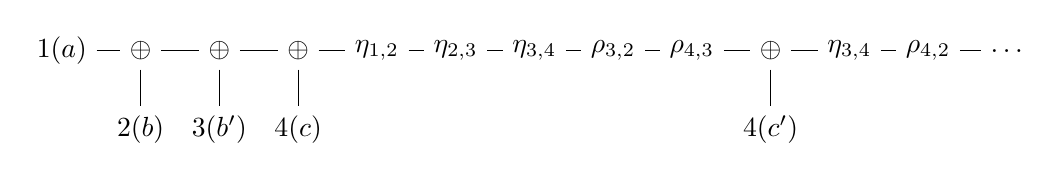
\begin{tikzpicture}[node distance={10mm}]
            \node (1) {$1(a)$};
            \node (2) [right of=1] {$\oplus$};
            \node (222) [below of=2] {$2(b)$};
            \node (3) [right of=2] {$\oplus$};
            \node (333) [below of=3] {$3(b')$};
            \node (4) [right of=3] {$\oplus$};
            \node (444) [below of=4] {$4(c)$};
            \node (5) [right of=4] {$\eta_{1,2}$};
            \node (6) [right of=5] {$\eta_{2,3}$};
            \node (7) [right of=6] {$\eta_{3,4}$};
            \node (8) [right of=7] {$\rho_{3,2}$};
            \node (9) [right of=8] {$\rho_{4,3}$};
            \node (10) [right of=9] {$\oplus$};
            \node (100) [below of=10] {$4(c')$};
            \node (11) [right of=10] {$\eta_{3,4}$};
            \node (12) [right of=11] {$\rho_{4,2}$};
            \node (13) [right of=12] {$\ldots$};
            \draw (1) -- (2) -- (3) -- (4) -- (5) -- (6) -- (7) -- (8) -- (9) -- (10) -- (11) -- (12) -- (12) -- (13); 
            \draw (2) -- (222) (3) -- (333) (4) -- (444) (10) -- (100);
        \end{tikzpicture}

        \vspace{1em}

        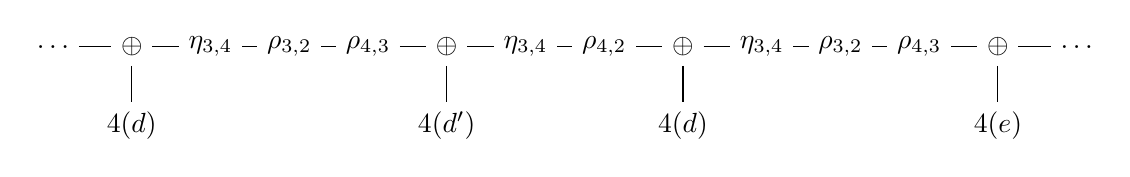
\begin{tikzpicture}[node distance={10mm}]
            \node (0) {$\ldots$};
            \node (13) [right of=0] {$\oplus$};
            \node (133) [below of=13] {$4(d)$};
            \node (14) [right of=13] {$\eta_{3,4}$};
            \node (15) [right of=14] {$\rho_{3,2}$};
            \node (16) [right of=15] {$\rho_{4,3}$};
            \node (17) [right of=16] {$\oplus$};
            \node (177) [below of=17] {$4(d')$};
            \node (18) [right of=17] {$\eta_{3,4}$};
            \node (19) [right of=18] {$\rho_{4,2}$};
            \node (20) [right of=19] {$\oplus$};
            \node (200) [below of=20] {$4(d)$};
            \node (21) [right of=20] {$\eta_{3,4}$};
            \node (22) [right of=21] {$\rho_{3,2}$};
            \node (23) [right of=22] {$\rho_{4,3}$};
            \node (24) [right of=23] {$\oplus$};
            \node (244) [below of=24] {$4(e)$};
            \node (25) [right of=24] {$\ldots$};
            \draw (0) -- (13) -- (14) -- (15) -- (16) -- (17) -- (18) -- (19) -- (20) -- (21) -- (22) -- (23) -- (24) -- (25);
            \draw (13) -- (133) (17) -- (177) (20) -- (200) (24) -- (244);
        \end{tikzpicture}

        \vspace{1em}

        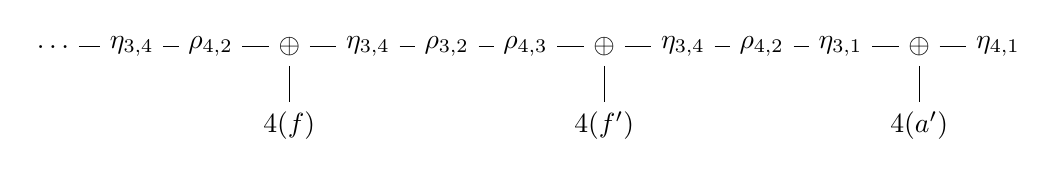
\begin{tikzpicture}[node distance={10mm}]
            \node (0) {$\ldots$};
            \node (25) [right of=0] {$\eta_{3,4}$};
            \node (26) [right of=25] {$\rho_{4,2}$};
            \node (27) [right of=26] {$\oplus$};
            \node (277) [below of=27] {$4(f)$};
            \node (28) [right of=27] {$\eta_{3,4}$};
            \node (29) [right of=28] {$\rho_{3,2}$};
            \node (30) [right of=29] {$\rho_{4,3}$};
            \node (31) [right of=30] {$\oplus$};
            \node (311) [below of=31] {$4(f')$};
            \node (32) [right of=31] {$\eta_{3,4}$};
            \node (33) [right of=32] {$\rho_{4,2}$};
            \node (34) [right of=33] {$\eta_{3,1}$};
            \node (35) [right of=34] {$\oplus$};
            \node (355) [below of=35] {$4(a')$};
            \node (36) [right of=35] {$\eta_{4,1}$};
            \draw (0) -- (25) -- (26) -- (27) -- (28) -- (29) -- (30) -- (31) -- (32) -- (33) -- (34) -- (35) -- (36);
            \draw (27) -- (277) (31) -- (311) (35) -- (355);
        \end{tikzpicture}
    \end{center}
    Thus, in this $k$-expression we use at most $4$ labels, and it constructs $\sunlet$. Thus $\cw(\sunlet) \leq 4$ as required.
\end{solution}
\end{parts}